\documentclass[xcolor=dvipsnames,compress]{beamer}

\usepackage{verbatim}
\usepackage{shortlst}
\usepackage{amssymb}
\usepackage{ccicons}
\usepackage[absolute,overlay]{textpos}
%\usepackage{pstricks}
\usepackage{graphicx} 
\usepackage{hyperref}                  
\usepackage{minted}                     

%%%%%%%%%%%%%%%%%%%%%%%%%%%%%%%%%%%%%%%%%%%%%%%%%%%%%%%%%%%%%%%%%%%%%%%%%%%%%%%%
% global beamer options
%%%%%%%%%%%%%%%%%%%%%%%%%%%%%%%%%%%%%%%%%%%%%%%%%%%%%%%%%%%%%%%%%%%%%%%%%%%%%%%%
\usetheme{Warsaw}
\usecolortheme[RGB={180,20,30}]{structure} 
\setbeamertemplate{items}[triangle] 
\setbeamertemplate{blocks}[rounded][shadow=true]
\setbeamertemplate{section in toc}[square]
\setbeamertemplate{subsection in toc}[square]
%\setbeamercovered{dynamic}
\setbeamercolor{framesource}{fg=gray}
\setbeamerfont{framesource}{size=\tiny}

%%%%%%%%%%%%%%%%%%%%%%%%%%%%%%%%%%%%%%%%%%%%%%%%%%%%%%%%%%%%%%%%%%%%%%%%%%%%%%%%
% hyperref options
%%%%%%%%%%%%%%%%%%%%%%%%%%%%%%%%%%%%%%%%%%%%%%%%%%%%%%%%%%%%%%%%%%%%%%%%%%%%%%%%
% currently not working :(
\definecolor{links}{HTML}{2A1B81}
\hypersetup{colorlinks,linkcolor=,urlcolor=links}

%%%%%%%%%%%%%%%%%%%%%%%%%%%%%%%%%%%%%%%%%%%%%%%%%%%%%%%%%%%%%%%%%%%%%%%%%%%%%%%%
% minted options (located at ~/texmf/tex/latex/local/minted.sty)
%%%%%%%%%%%%%%%%%%%%%%%%%%%%%%%%%%%%%%%%%%%%%%%%%%%%%%%%%%%%%%%%%%%%%%%%%%%%%%%%
\usemintedstyle{tango}
% seems we need this for add a label to framed code (fancyvrb - minted issue)
\makeatletter
\minted@define@extra{label}
\makeatother

\newminted{c}{gobble=4,fontsize=\tiny,frame=single,rulecolor=\structure}
%\newminted{make}{gobble=4,fontsize=\tiny,frame=single,rulecolor=\structure}
%\newminted{sh}{gobble=4,fontsize=\tiny,frame=single,rulecolor=\structure}
\newminted{cpp}{gobble=4,fontsize=\tiny,frame=single,rulecolor=\structure}
\newminted{xml}{gobble=4,fontsize=\tiny,frame=single,rulecolor=\structure}
%\newminted{sql}{gobble=4,fontsize=\tiny,frame=single,rulecolor=\structure}
\newminted{py}{gobble=4,fontsize=\tiny,frame=single,rulecolor=\structure}

% reserved characters reminder:
% # $ % ^ & _ { } ~ \

%%%%%%%%%%%%%%%%%%%%%%%%%%%%%%%%%%%%%%%%%%%%%%%%%%%%%%%%%%%%%%%%%%%%%%%%%%%%%%%%
% commands and environments
%%%%%%%%%%%%%%%%%%%%%%%%%%%%%%%%%%%%%%%%%%%%%%%%%%%%%%%%%%%%%%%%%%%%%%%%%%%%%%%%
% reference section
\newenvironment{reference}[2]{% 
    \begin{textblock*}{\textwidth}(#1,#2) 
    \tiny\it\bgroup\color{blue}}{\egroup\end{textblock*}} 

% vi fonts
\newcommand\Fontvi{\fontsize{6}{7.2}\selectfont}
% vi blocks
\newenvironment{vi}{%
    \Fontvi\verbatim}{\endverbatim}

% has some problem
\newcommand{\inlineitem}{%
    \leavevmode\usebeamertemplate{itemize item}\hspace{.5em}}

% credit of images
\newcommand{\source}[1]{\begin{textblock*}{4cm}(8.7cm,8.6cm)
    \begin{beamercolorbox}[ht=0.5cm,right]{framesource}
        \usebeamerfont{framesource}\usebeamercolor[fg]{framesource} Source: {#1}
    \end{beamercolorbox}
\end{textblock*}}



\title[dbus]{Interprocess Communication with DBus}
\subtitle{An introduction}
\author{Alexandre Moreno}
\institute[Seenergy]{SEEnergy Corp.\\
   \texttt{alexandre@seenergy.com.tw}
} 
\subject{talk}
\date{\today}
%\logo{\includegraphics[height=1.0cm]{../Company_Logo.png}}
\titlegraphic{\ccbysa}

\begin{document}

\begin{frame}[plain]
   \titlepage
\end{frame}

\section*{outline}
\begin{frame}
   \tableofcontents
\end{frame}

\section[intro]{Introduction}
\begin{frame}
    \frametitle{What is D-Bus?}
    "D-Bus is a message bus system, a simple way for applications to talk to one another. In addition to interprocess communication, 
    D-Bus helps coordinate process lifecycle; it makes it simple and reliable to code a "single instance" application or daemon, 
    and to launch applications and daemons on demand when their services are needed."\\
    \hspace*{\fill} \structure{dbus.freedesktop.org}\\~\\
    DBus can be thought as a middleware for easily managing processes and devices.\\~\\
    It performs even on devices with relatively low computing power, such as cost sensitive embedded platforms.\\~\\
\end{frame}

\begin{frame}
    \begin{reference}{4mm}{85mm}
    * A binding is just a wrapper of the C reference implementation of the D-Bus protocol. There are projects that reimplement the protocol, e.g. Java, D-Bus Sharp (.NET)
    \end{reference}
    Platform support:
    \begin{itemize}
    \item Linux, most unices and also a \structure{Windows} port
    \end{itemize}
    Source:
    \begin{itemize}
    \item Latest stable release: \href{http://dbus.freedesktop.org/releases/dbus/dbus-1.6.8.tar.gz}{D-Bus 1.6.8} (2012-09-28)
    \end{itemize}
    License:
    \begin{itemize}
    \item GPL or Academic Free License 2.1
    \end{itemize}
    Language/framework support:
    \begin{itemize}
    \item Bindings* to C++, Java, Python, Qt, GLib, Objective-C\\
    \href{http://www.freedesktop.org/wiki/Software/DBusBindings}
    {http://www.freedesktop.org/wiki/Software/DBusBindings}
    \end{itemize}
\end{frame}

\begin{frame}
    D-Bus is not intended to be used for bulk data transfer.\\~\\
\end{frame}

\begin{frame}[fragile]
    \frametitle{Projects using DBus...}
    ...that I can think of
    \begin{itemize}
    \item GNOME and KDE (desktop environments)
    \item systemd, Upstart, etc.
    \item UDisks, UPower
    \item Lots of media players
    \item BlueZ, wpa\_supplicant
    \item GENIVI (automotive Linux)
    \item Tizen (MeeGo cont.)
    \end{itemize}
\end{frame}



\section[lib]{libdbus}
\begin{frame}
    \frametitle{Low-level API}
    A core concept of the D-Bus implementation is that \structure{libdbus} is intended to be a low-level API. 
    Think of using Xlib/DirectFB directly, instead of Qt/GTK+.\\~\\
    The rationale is that an IPC system API should not "leak" all over a program; 
    it should come into play only just before data goes over the wire.\\~\\
    Despite it is recommended to use one of the many bindings available (GLib, Qt, Python, Mono, Java, etc.)
    we will look briefly at the libdbus API.
\end{frame}
\begin{frame}
    The two core data types in libdbus are:
    \begin{itemize}
    \item \structure{DBusMessage}: the most basic unit of communication over the bus, that conveys either 
    a method call, method reply, error reply or signal
    \item \structure{DBusConnection}: represents a connection to another application, a stream of messages
    send/receive to/from a remote application
    \end{itemize}
\end{frame}
\begin{frame}
    \frametitle{Integration with the main loop}
\end{frame}

\begin{frame}[fragile]
    \frametitle{Example: DBus service using blocking API}
    \begin{ccode}
    /* returns TRUE if disconnect message has not been processes */
    while (dbus_connection_read_write_dispatch(connection, -1));
    \end{ccode}
\end{frame}

\begin{frame}
    \frametitle{Example: DBus client using low-level API}
\end{frame}

\section[protocol]{Protocol Concepts}

\begin{frame}
    \frametitle{Message Bus}
    The core D-Bus protocol is a 2-way, asynchronous, binary protocol.\\~\\
    While it is possible to use for direct application to application communication (using libdbus), 
    the most common usage of the protocol is via a message bus daemon.\\
    There are two standard message bus instances:
    \begin{columns}[t]
    \begin{column}{0.5\textwidth}
    %\minipage[c][0.5\textheight][s]{\columnwidth}
    \begin{itemize}
    \item \structure{system bus}
    \item \structure{session bus}\\~\\
    \end{itemize}
    %\vfill
    It is also possible to use a custom bus, by writing a different bus config file (man dbus-daemon).
    %\endminipage
    \end{column}
    \begin{column}{0.5\textwidth}
    \begin{center}
    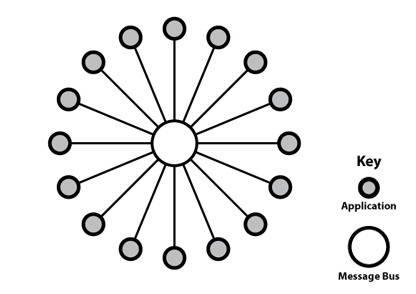
\includegraphics[width=0.95\textwidth]{bus.png}
    \source{Google.com}
    \end{center}
    \end{column}
    \end{columns}
\end{frame}

\begin{frame}
    \frametitle{System Message Bus}
    The system bus, is commonly used for notification of system changes, such as devices added or removed (udev).\\~\\
    Typically system daemons abstract device management (e.g. storage management with udisks), and provide a DBus interface to applications.
    This daemons use libudev to monitor status of hardware, and signal changes to interested applications.\\~\\
    \begin{block}{}
        kernel $\Rightarrow$  udev $\Rightarrow$ subsystem daemon $\Leftrightarrow$ DBus $\Leftrightarrow$ applications
    \end{block}
\end{frame}

\begin{frame}
\frametitle{Messages-oriented Protocol}
    D-Bus works by sending messages between processes. There are 4 message types: 
    \begin{itemize}
    \item \structure{Method call}: ask to invoke a method on an object.
    \item \structure{Method return}: return the results of invoking a method.
    \item \structure{Error return}: an exception caused by invoking a method.
    \item \structure{Signal}: notifications that an event has occurred.\\~\\
    \end{itemize}
    If you're using a sufficiently high-level binding, you may never work with messages directly.
\end{frame}

\begin{frame}
    Messages contain a header and a body, and both parts make use of the DBus Type System for marshalling the data:
    \begin{itemize}
    \item The header is processed by the message delivery system (the bus daemon), and 
    \item The body is interpreted by the recipient of the message.
    \end{itemize}
\end{frame}

\begin{frame}
    \frametitle{Primitive Types}
    TODO: Detail basic types
\end{frame}

\begin{frame}
    \frametitle{Compound Types}
    \begin{itemize}
    \item \structure{array}: a variable-length sequence of the same type 
    \item \structure{struct}: a fixed-length sequence whose members may have different types
    \item \structure{dictionary}: a mapping from values of the same basic type to values of the same type 
    \item \structure{variant}: a container which may hold any D-Bus type, including another variant.
    \end{itemize}
\end{frame}
\begin{frame}
    \frametitle{Introspection Data Format}
    DBus objects may be introspected at runtime (by implementing org.freedesktop.DBus.Introspectable), returning an XML string that describes the object.\\~\\ 
    The same XML format may be used in other contexts as well, for example as an \structure{Interface Design Language} (IDL) for generating static language bindings.\\~\\
    An example of this is shown later.
\end{frame}
\begin{frame}[fragile]
    \frametitle{IDF XML Interface example}
    \begin{xmlcode}
    <node>
        <interface name="tw.com.seenergy.demo">
            <method name="SayHello">
                <annotation name="com.trolltech.QtDBus.QtTypeName.In1" value="QVariantMap"/>
                <arg name="name" type="s" direction="in"/>
                <arg name="customdata" type="a{sv}" direction="in"/>
            </method>
            <method name="SayBye"/>
            <property name="Hello" type="y" access="readwrite"/>
            <signal name="SomebodySaidHello">
                <arg name="who" type="s"/>
            </signal>
        </interface>
    </node>
    \end{xmlcode}
\end{frame}

\begin{frame}
    \frametitle{Custom Types}
    IDF elements may have \structure{annotations}, which are generic key/value pairs of metadata.\\~\\
    They are similar conceptually to Java's annotations and C\# attributes.
\end{frame}

\begin{frame}
    \frametitle{DBus service activation}
\end{frame}

\section[design]{DBus Interfaces}

\begin{frame}[fragile]
    \frametitle{Standard Interfaces}
    \begin{itemize}
    \item \structure{org.freedesktop.DBus.Introspectable}
    \end{itemize}
    This interface has one method:
    \begin{vi}
        org.freedesktop.DBus.Introspectable.Introspect (out STRING xml_data)
    \end{vi}
    This method returns an XML description of the object, 
    including its interfaces (with signals and methods), objects below it in the object path tree, and its properties.
    
    \begin{itemize}
    \item \structure{org.freedesktop.DBus.Properties interface}
    \end{itemize}
    Many native APIs will have a concept of object properties or attributes. 
    \begin{vi}
        org.freedesktop.DBus.Properties.Get (in STRING interface_name,
                                            in STRING property_name,
                                            out VARIANT value);
        org.freedesktop.DBus.Properties.Set (in STRING interface_name,
                                            in STRING property_name,
                                            in VARIANT value);
        org.freedesktop.DBus.Properties.GetAll (in STRING interface_name,
                                            out DICT<STRING,VARIANT> props);
    \end{vi}
\end{frame}

\section[web]{Web Clients}

\begin{frame}
    \frametitle{Web Applications}
    \begin{itemize}
    \item\href{http://sandbox.movial.com/wiki/index.php/Browser_DBus_Bridge}
    {Browser DBus Bridge}: JavaScript D-Bus bindings implementation for web browsers
    \item\href{http://www.pengutronix.com/software/json-dbus-bridge/index_en.html}
    {JSON-D-BUS-Bridge}: a \href{http://www.fastcgi.com/devkit/doc/fastcgi-whitepaper/fastcgi.htm}{FastCGI} application that provides access to D-Bus.
    \end{itemize}
\end{frame}

\begin{frame}
    \frametitle{JSON-DBus Bridge}
    \begin{itemize}
    \item Translates JSON-RPC (as used in the AJAX framework \href{http://manual.qooxdoo.org/1.6/pages/communication/rpc.html}{qooxdoo}) 
    calls to DBus messages, and viceversa.
    \item Currently there are some limitations, most notably DBus signals are not supported
    \end{itemize}
\end{frame}

\section[ex]{Examples}

\begin{frame}[fragile]
    \frametitle{Generic Accessor - No Proxy Object}
    It is  also possible, and sometimes desirable, to directly place calls to remote objects:
    \begin{cppcode}
        QDBusInterface remoteApp( "com.example.Calculator", "/Calculator/Operations",
                               "org.mathematics.RPNCalculator" );
        remoteApp.call( "PushOperand", 2 );
        remoteApp.call( "PushOperand", 2 );
        remoteApp.call( "ExecuteOperation", "+" );
        QDBusReply<int> reply = remoteApp.call( "PopOperand" );

        if ( reply.isValid() )
            printf( "%d", reply.value() );          // prints 4
    \end{cppcode}

\end{frame}

\begin{frame}
    \frametitle{NVRManager}
    To study whether DBus is suitable for our system, we will develop a case study, covering the following bits:
    \begin{itemize}
    \item interface design: provide a \structure{programmatic} API for controlling NVR core services     
    \item a service implementing several related interfaces, and exporting several object paths
    \item client implementation of proxy object vs. direct access to an interface's methods/signals/properties
    \end{itemize}
\end{frame}

\begin{frame}
    \frametitle{NVRPlayer}
    Media handling: querying, recording, playback, etc.
\end{frame}

\end{document}
